% !TEX TS-program = xelatex
% !TEX encoding = UTF-8 Unicode

\providecommand{\home}{../..}
\documentclass[\home/main.tex]{subfiles}

\begin{document}

\chapter{Introduction}\label{ch:introduction}

% \textbf{High-level problem statement to draw in the reader:}
Robotics promises to relieve humanity from repetitive tasks. Yet, why is there currently no robot that ties our shoelaces, weeds our gardens, and folds our shirts?
These tasks break the boundaries of the scripted environment for which existing robot technologies are programmed. Programmed robots follow routines to assemble cars and weld miniaturized electrical components at astounding speeds and fine-grained precision. However, these robots operate in a cage where every instruction is precisely defined with minimal room for deviation. Nevertheless, when robots are supervised by humans, they can operate outside their cages. For example, the da Vinci\textregistered\ robot allows performing surgery by teleoperating robotic arms through a hand-operated console. However, there exist no adaptive cruise control for surgery yet.
Evidently, current robotic technologies contain an impressive repertoire of manipulation tasks solved within industrial or laboratory conditions.
Gracefully and productively adopting robots in our daily lives will significantly impact industry and society. Robots will sort and pack all types of objects in warehouses, install electrical wiring in our cars, helping elderly people dress, and clean up our houses.
\todo{Missen we hier het belang van dexterous manipulation niet?}
% VOORBEELDEN HIER als volgende zin
%     robot butler: is de was aan het plooien, voor oude mensen aan het zorgen, aan het opruimen, aan het koken 
%     industrie voorbeelden: sort and package objects, bake bread, clean-up the factory, replace eletrical wiring outside the international space station. 
%     probeer de voorbeelden zoveel mogelijk rond manipulatie te houden!

% \textbf{Overgang Relevantie deformable objects.}
For the robot butler to become a reality, control algorithms need to loosen assumptions about the environment in which robots operate. Nowadays, robotic manipulation solutions require environments to be fully specified and the object's configuration to be fixed. However, the real world presents an infinite supply of configurations. To find solutions for this problem, we study the robotic manipulation of objects that provide an infinite amount of configurations: deformable objects.

% Endowing robots with skills to handle objects that deform on interaction helps to solve a general problem: how should the robot react if the configuration changes.

\section{Deformable object manipulation and robotic laundry}
% what is it 
Many everyday objects deform upon force interaction: the wires we use to charge our phones, the clothes we carry, and the sutures doctors use for stitching wounds.
% Robot laundry
In this research, we consider the problem of \textbf{automating the task of folding clothing}. Folding clothing is part of the laundry cycle and a potential task for future household robots.
% \textbf{Hier kort over robotic laundry, het proces en waarom het moeilijk en interessant is. Eventueel economische cijfers toevoegen.}
% WAAROM ECONOMISCH + SOCIAAL
With aging populations, increasing quality of life and importance of work-life balance, automating dull and repetitive tasks in households merits benefits from a social and financial point of view. Outsourcing tasks to robots allows freeing up time or budget if a domestic helper is employed. For older people, or people with limited mobility, domestic task automation can give a feeling of independence as the need for assistance of home care workers is reduced.
Additionally, there is a significant portion of industry working with garments, textiles and other deformable objects that could also benefit from developments in general-purpose robotic automation.

% why is it relevant?
Although automating domestic tasks can free up a significant amount of time, developments in automation have primarily focussed on industrial automation. This is because industrial tasks are much simpler to automate compared to domestic environments where it is hard to exert exact control and enforce conditions. Even in research, folding clothing has received little attention. The main reason is that robotics research focuses primarily on grasping and manipulating rigid objects. Rigid objects do not deform during interaction and significantly reduce the required information. For example, grasping your morning cup of coffee requires only to know the position of the cup's handle.
On the contrary, if the handle is highly deformable, you also need to reason about its shape and how it deforms depending on the planned manipulation.
Comprehending why planning for deformations is challenging can be done by understanding why modern robots and their control algorithms fail.
% However, modern pick-and-place robots already experience difficulties grasping rigid objects that are partially hidden or transparent. We first look at why modern robots and their control algorithms fail. 

\section{Traditional control pipelines do not work for folding cloth}
A daily-life example found in common kitchens illustrates the workings of today's industrial robots. Instead of manually slicing food into smaller pieces for cooking, one\todo{"one" of "you"?} can use a food processor to automate the slicing process.
%\footnote{In the Dutch language, a kitchen robot is unluckily used as a term for kitchen appliances that perform actuated whisk, mix and knead operations.}
Using the food processor requires structuring the environment: one needs to equip the correct blade on the motor shaft, preprocess the food into a manageable size for the blade and feed it through the tube while activating the motor. Deviating from this setting can lead to minor failures and even harmful situations. For example, inserting oversized food slices might lead to motor stalling. More dangerously, there is no intelligence in consumer-grade appliances stopping the motor from turning the blades if you decide to insert your hand into the feeding tube.

Current robotic control pipelines are organized similarly to the given food processor example: structuring the environment and decomposing the problem. Decomposing a large problem into subproblems is a general problem-solving and engineering paradigm that allows making assumptions that simplify the solution strategy. In robotics, this modular approach is omnipresent and has led to incredible levels of automation and an increase in productivity \autocite{Graetz2018}. However, the innate fear that robots will soon take over our jobs \autocite{cave2019hopes} is unwarranted.
Open-loop control architectures with no adaptability towards deviations and failures elsewhere in the control pipeline will repeatedly fail when variations occur in the routine. Some of the most advanced robotics research and development teams demonstrate this in the 2015 DARPA Robotics Challenge Finals \autocite{DARPA2015}. The consequences of exposing robots to unstructured environments can be viewed in published video clips \autocite{darpaVideos}: million-dollar robots tumbling to the ground in, frankly, hilarious ways. In one example, a robot is supposedly turning a valve. However, the robot's walking path is misaligned, making it stand next to the valve instead of in front of it. Consequently, the robot is performing a rotating movement with its arm in thin air while assuming resistance of the valve for balancing. The missing counterbalance makes the robot falls to the ground. The rotating valve failure brings the inner working of control loops to light: a sequence of isolated modules that solve decomposed tasks with minimal regard for failures down- or upstream in the pipeline.
% This is frappant considering with how much apparent ease humans solve similar tasks. 

Robots that manipulate deformable objects employ similar pipelines: a sequence of modules with functionalities ranging from garment type identification to corner point detection and executing preprogrammed folding sequences. We visualize a canonical pipeline for folding clothing in \cref{fig:intro_canonical_control_pipeline}. These approaches are assumption-heavy and can have limited generalization. Engineered pipelines also have difficulty scaling: successful implementations require 24 minutes to fold a single shirt \autocite{Maitin2010}. This motivates our research to look in the direction of \emph{employing learning-based methods} to create autonomous systems that can perform robust grasp synthesis when faced with the high amount of variations that occur in the real world.

\begin{figure}
    \centering
    \subfile{figures/fig-canonical-manipulation-pipeline-folding.tex}
    \caption{TODO MAAK FIGUUR. Canonical robotic control pipeline for folding clothing. Each module solves an isolated task and passes the result to the next module.}
    \label{fig:intro_canonical_control_pipeline}
\end{figure}

\section{From engineered pipelines to end-to-end learning}
Machine learning is a subset of \gls{AI} methods that can learn patterns from examples. The successes of deep neural networks, a machine learning method, in playing Atari video games \autocite{Mnih2015} and beating human champions in the game of Go \autocite{gaemofGo2016}, has driven robotics researchers to adopt machine learning across the whole pipeline. This led to an end-to-end learning approach in which the robot has to figure out how to move its arms using a single camera image. Every functional module in the pipeline on the top in \cref{fig:intro_end2end}, for example, is integrally replaced with a deep neural network.

Unfortunately, end-to-end learning for robotics is privileged to organizations containing massive computational power and expensive robotic farms. The robots in these farms operate \emph{interactively} in an environment: they perform actions by trial-and-error to maximize a predefined success criteria. Although robots learning from scratch yields entertaining footage, similar to the falling robots of DARPA 2015, it tires quickly as learning from scratch on a real robot takes tremendous amounts of time and is potentially unsafe. From the perspective of how humans learn, it makes no sense to have a system learn from scratch. Imagine asking a human baby to do the laundry while it still has to learn how to move its limbs. If we want physical systems to solve tasks in dynamic environments, they require some form of prior knowledge to accelerate learning.

For cloth folding robots, we have on the one hand robots that use engineered pipelines and take 24 minutes to fold a shirt \autocite{Maitin2010}. On the other hand, there exist robots that learn to fold from scratch but require over \qty{100000}{} physical robot-environment interactions \autocite{Matas2018}. In this research, we explore solutions that lie in the middle between the modelling and learning paradigm.

%  This slow learning time motivates our research to accelerate robot learning for folding clothing. 

% deze robots worden dan in een RL framework geplaatst waar ze moeten interageren. Dit zou nog grappigere beelden oplveren dan DARPA 2015: robots dat zich niet bewust zijn van hun ledematen moeten hun motoren leren aansturen om bv kledij te vouwen. Imagine the situations. Although, most robots would probably fall down quickly and harm themselves in the process. 
% \emph{This motivates our research to democratize robotics by accelerating robotic learning.}

\begin{figure}[htpb]
    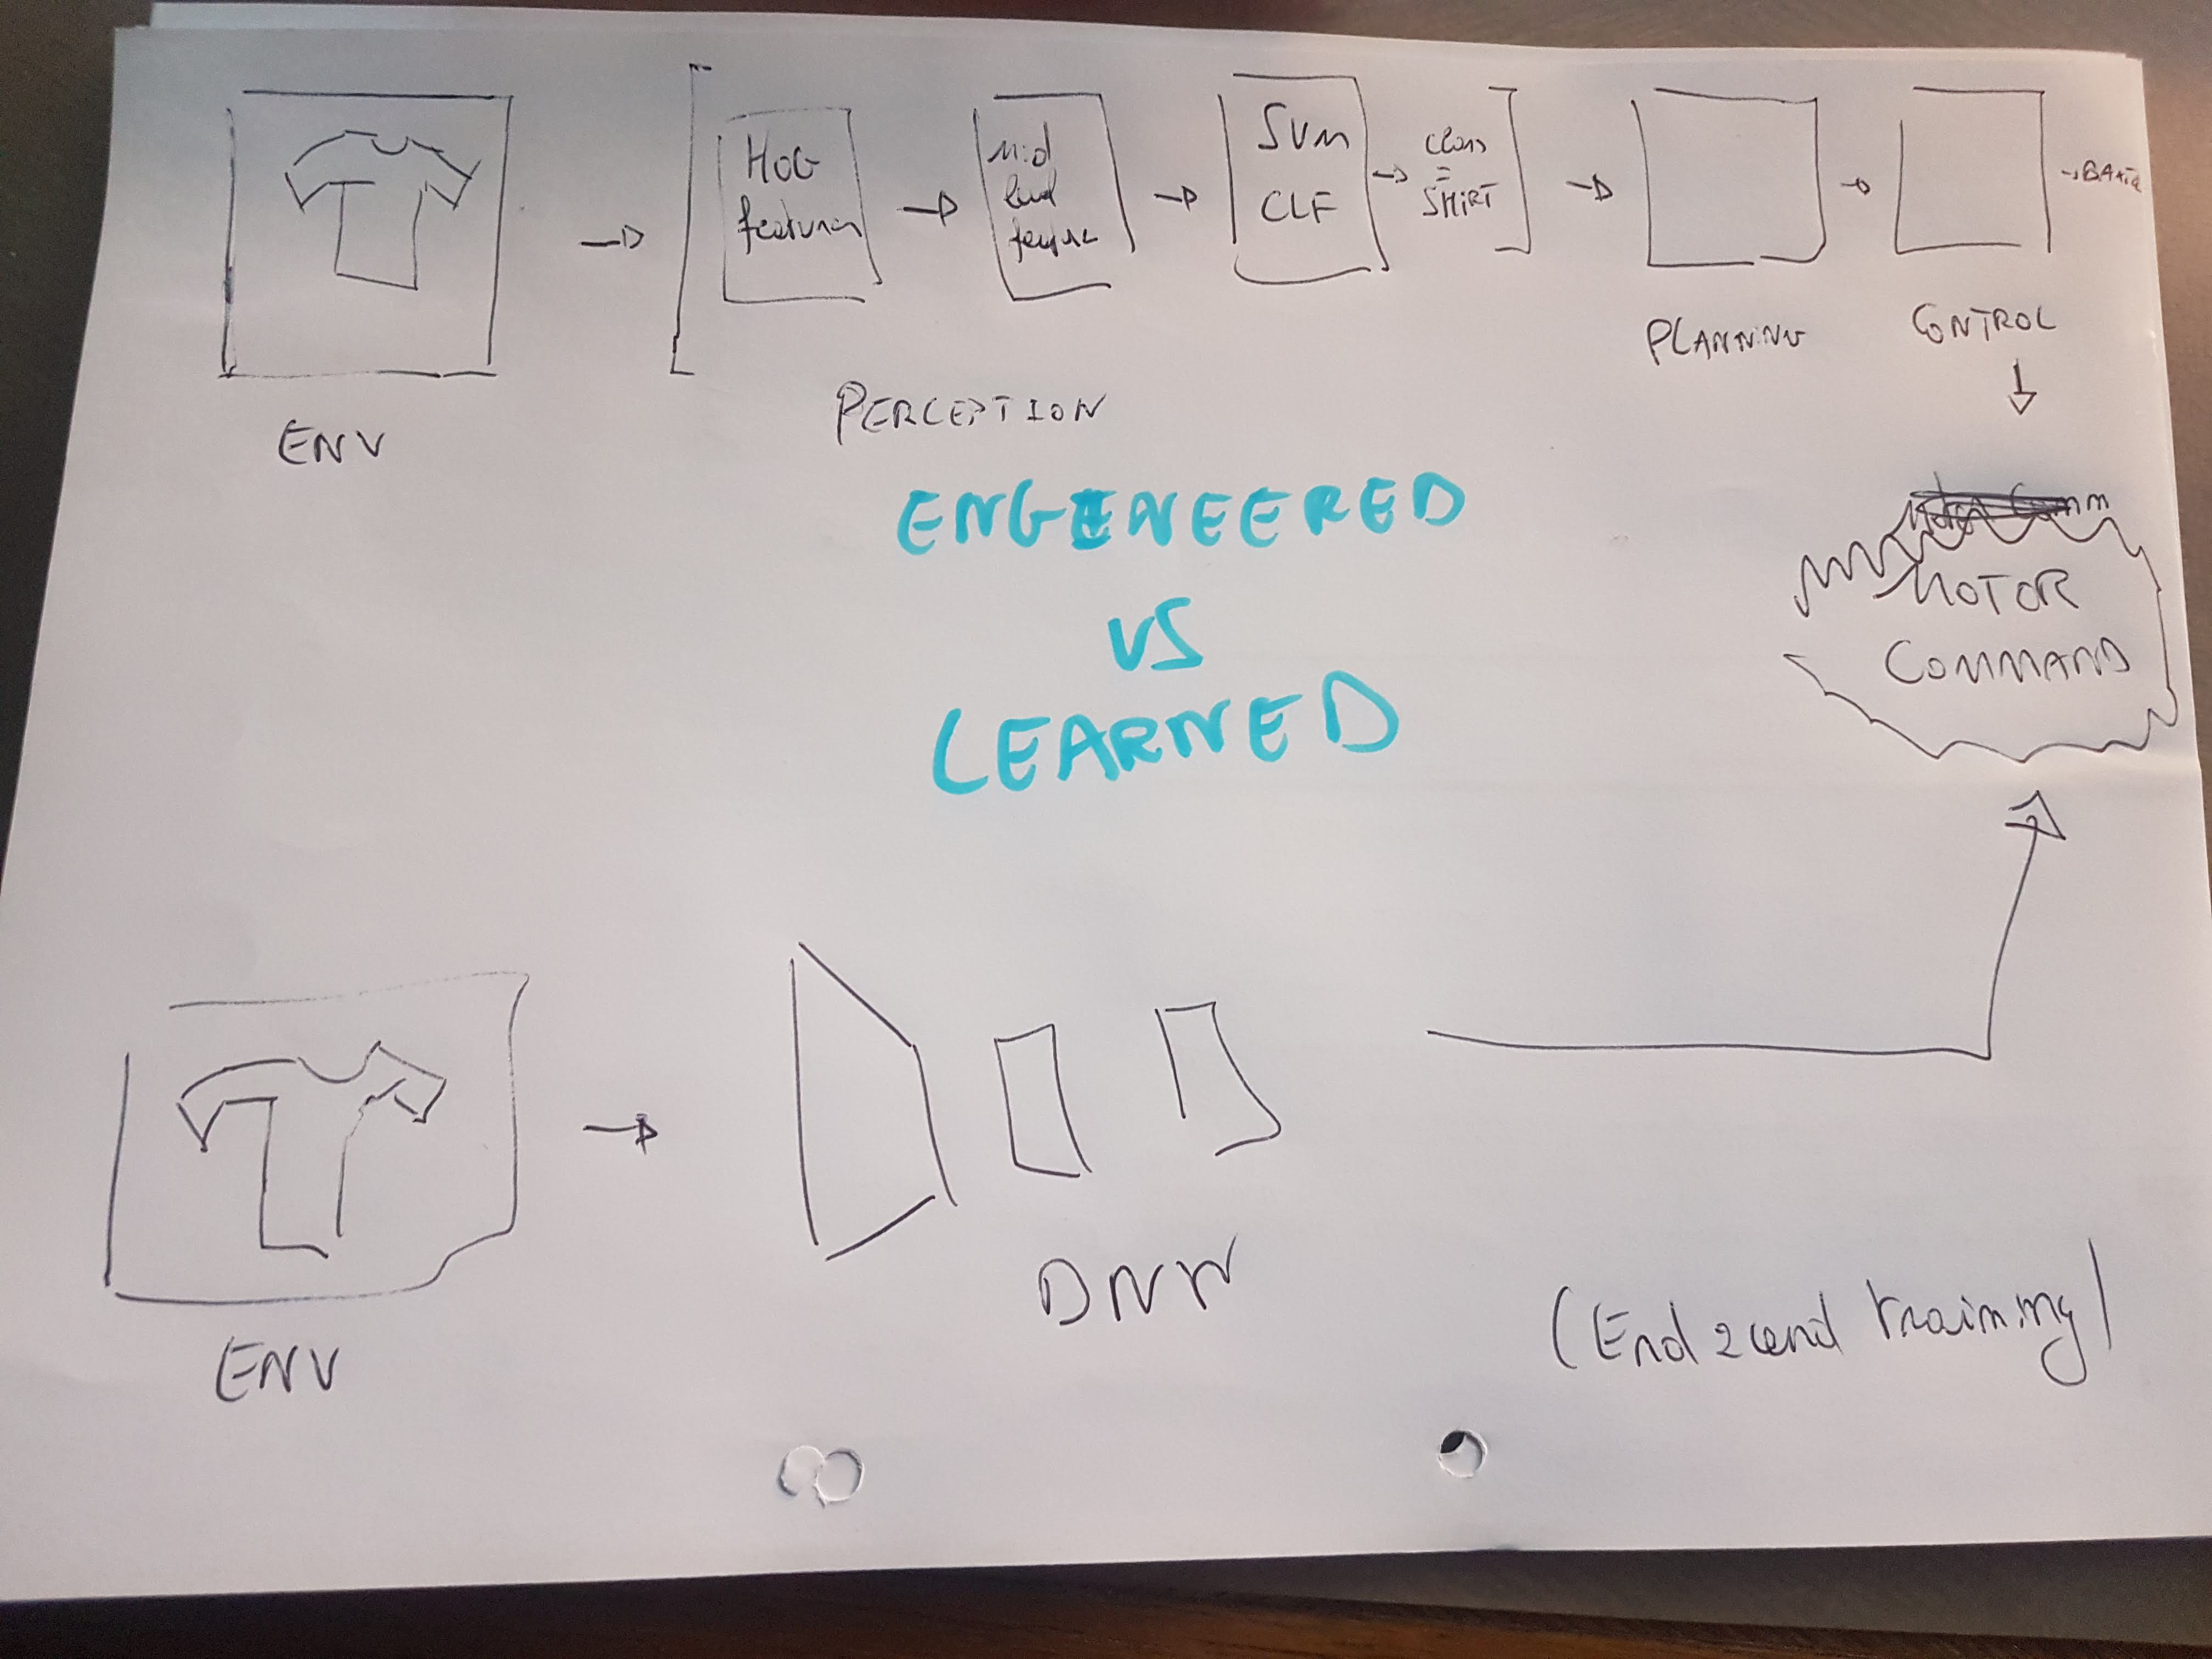
\includegraphics[width=\linewidth]{\home/chapters/01-introduction/figures/end2end-mockup}
    \caption{\textbf{Standard robotic control pipelines versus end-to-end architectures.} The diagram on the top shows how an image is processed to manually tuned features in order to do state estimation. This is then used downstream for trajectory planning and motor control. The diagram on the bottom shows an end-to-end approach to the same problem: an image is given to a deep neural network that learns its own features and executes actions directly on the actuators.}
    \label{fig:intro_end2end}
\end{figure}

\section{Accelerating learning of robotic manipulation of deformable objects}
Learning is considered to be a central component for autonomous systems to deal with real-world variability \autocite{kroemer2021review}. For real robots to learn to fold clothing articles, we research the following four areas:
(i) generation of cloth folding datasets for learning;
(ii) using simulations as a safe and fast environment for learning;
(iii) facilitating state estimation of cloth; and
(iv) understanding task intent rather than copying human behaviour.
We discuss these areas in the following sections.

%  TODO: YOU ARE HERE.
%  Deze stukjes nog uitschrijven (datasets, simulation). En dan research outline kort aanvullen. Zie bv thesis van Olivier. Dat moet kort zijn. 
\subsection{Datasets}
A critical piece of the puzzle for building intelligent systems comes in the form of \emph{data}. The standard paradigm in machine learning is to provide a dataset with, for example, images of folded and unfolded shirts and train a model that learns to distinguish between the two. Datasets with task demonstrations have enabled training autonomous driving cars \autocite{bojarski2016end}, learning quadruped robotic locomotion \autocite{peng2020learning}, drone flight \autocite{Giusti2016} and learning to dishes in a plate rack \autocite{Finn2016}. However, in the field of  learning robotic manipulation skills for clothing, no dataset with example demonstrations of people folding clothing exist. 

\subsection{Simulation}
Whereas real dataset generation can be expensive to obtain, synthetic data allows generating massive datasets and quick experimentation.

\subsection{Instrumentation}
When we use our hands to crush a plastic cup, multiple sensors of our body activates: we use our eyes to observe the deformations, our ears register the amplitude of the impact, our hands notify us of how much force we are applying, and our proprioceptive system signal us how much our hand is closed. This rich interplay of multiple modalities in the human cognitive system is in stark contrast to robotic manipulation pipelines that are primarily vision-based. Vision is important for robotic manipulation: it helps infer the object location relative to the robot end-effectors, it helps understand the object's geometry and some of its physical properties. Furthermore, commercial cameras are readily available and accessible compared to other sensors such as tactile sensors. Nevertheless, considering the giant leaps of object recognition using deep learning, robots still struggle to recognize objects in more difficult contexts such as partial occlusion, transparent object and moving objects \autocite{Guo2014,sajjan2019cleargrasp,Ojha2015}.
Incorporating heterogeneous sources of information can alleviate problems when state estimation cannot be directly observed from pixels. For example, finding the occluded corner of a crumbled towel is possible using sensing and simplifies the folding process considerably.
We denote the process of adding sensory information to the learning environment of a robot as \textbf{instrumentation}. The goal is to direct the large focus on using vision-based state estimation to applying other sensor modalities in the environment such as tactile sensing in a cloth and force sensing in the fingers. Our hypothesis is that some modalities encode parts of the state in a compacter way than vision. This semantically more meaningful encoding accelerates learning, which is important in robotics where real rollouts are expensive.

% \subsection{Grippers for folding}
% The human hand is a general-purpose manipulator with formadiable dexterous manipulation capabilities. 
\subsection{Understanding task intent}
Humans their ability to infer task intent from demonstration is in stark contrast to imitation learning approaches from the machine learning field. Imitation learning for autonomous cars, for example, answers the question \enquote{how many degrees would a human driver move the steering wheel now that this tree is in front of me?}. Although the correct answer is probably avoiding to come into the situation that a tree is front of the car, no human driver would likely be able to provide an exact answer.

Instead of creating a dataset of task scenarios with associated human actions, the interactive trial-and-error approach of \gls{RL} shares more semantics with learning from a human perspective. For example, humans encourage desirable behaviour in dogs by means of treats or punishment. In this example, the snack is the reward signal. Applying the idea of reward and punishment to robotics is a popular learning approach but requires finding the appropriate reward signal. In the case of cloth folding, it is ambiguous to write down a mathematical formula that describes how well a person is folding a clothing article. How does one quantify the number of wrinkles to a performance measure? Does it matter that a folded towel does not contain perfectly straight lines? What is the definition of a folded shirt? Finding a reward signal requires identifying, measuring and quantifying all aspects of performance. This might not be possible for all problems, like cloth folding.

% Infants are considered to have a different internal learning loop compared to dog training.
Compared to training dogs, infants are known to understand task intent behind human behaviour without requiring explicit reward signals \autocite{warneken2006altruistic}.
We argue that a similar approach can be applied for the case of robotic folding, and learning in general. By learning the reward function from human demonstrations, without labelling, one can use this reward signal in an \gls{RL} setting. This idea is generally known as inverse \gls{RL}. However, inverse RL learns a reward function in conjunction with learning how to behave. We propose decoupling this process and learning a reward function separately to speed-up training and use it for other applications like process monitoring.

\section{Research outline}
Our main goal is to investigate how learning-based approaches can be accelerated for . We focus exclusively on the application of robotic manipulation of cloth.

Simulation-driven approach
Dataset with people folding clothing
Low-cost robot setup to fold cloth in-vivo
Instrumentation
Self-supervised reward function

\section{Publications}

\end{document}
